\documentclass[11pt]{article}
\usepackage{graphicx}
\usepackage{hyperref}
\usepackage[dvipsnames, svgnames, x11names, hyperref]{xcolor}
\hypersetup{
	colorlinks,
	citecolor=Violet,
	linkcolor=Red,
	urlcolor=Blue}
\usepackage{natbib}

\setlength{\textwidth}{6.5in}
\setlength{\headheight}{0in}
\setlength{\textheight}{8.0in}
\setlength{\hoffset}{0in}
\setlength{\voffset}{0in}
\setlength{\oddsidemargin}{0in}
\setlength{\evensidemargin}{0in}


\title{Homework 6 Solution}

\author{Nana Ama Nyamekye Darpaah}

\begin{document}
	
	\maketitle
	This is my GitHub link: \href{https://github.com/nnd2016/phys-ga2000.git}{Nana Ama's GitHub Link}
	
	\section{Question 1}
	A plot of the data of first 4 galaxies is as shown in Figure \ref{fig:galaxy_plots}.  we From the plot, see that the peaks of all the graphs were around 660nm which corresponds to the absorption spectra of hydrogen at the red wavelength of 656nm.
	
	\begin{figure}[!htb]\begin{center} 
			\vspace{12pt}
			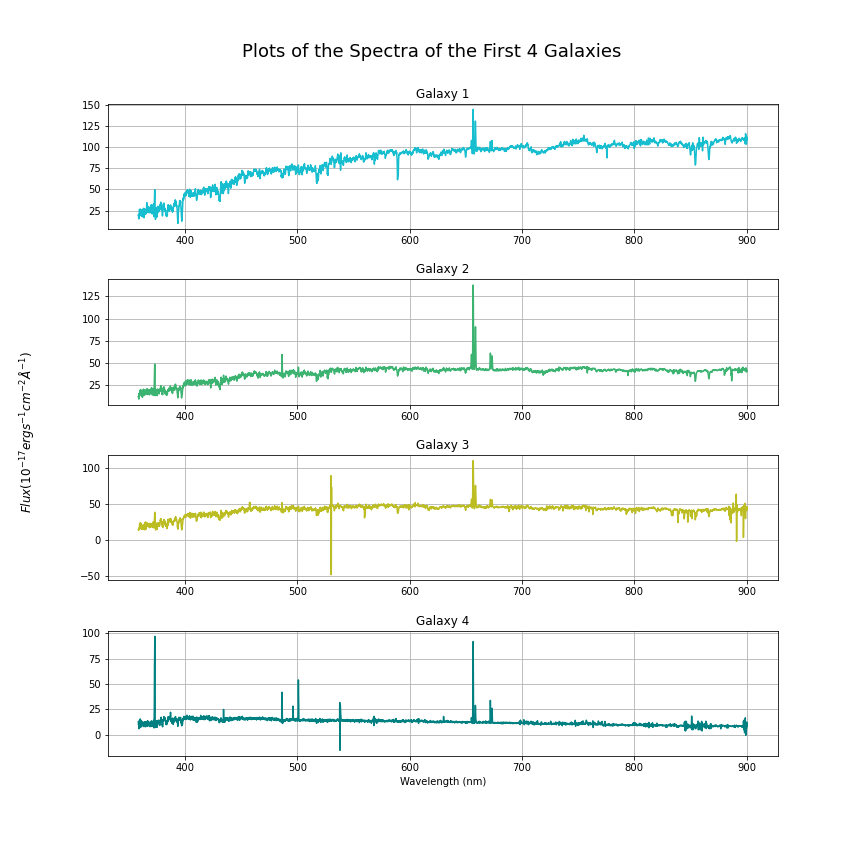
\includegraphics[width=0.9\textwidth]{galaxy_plots.png}
			\caption{A plot of first 4 galaxies of the data }
			\label{fig:galaxy_plots} 
		\end{center}
	\end{figure}

	The eigenvalues and eigenvectors were found with both Singular Value Decomposition(SVD) and the Covariance Matrix. The condition number of C was found to be -335542944.0 and that of R was 43057768562688.0. SVD is better in the sense that singular values are more numerical stable than eigenvalues.
	\\
	The first 5 eigenvectors were determined and plotted as shown in Figure \ref{fig:eigenvector_plots}.
	
	\begin{figure}[!htb]\begin{center} 
			\vspace{12pt}
			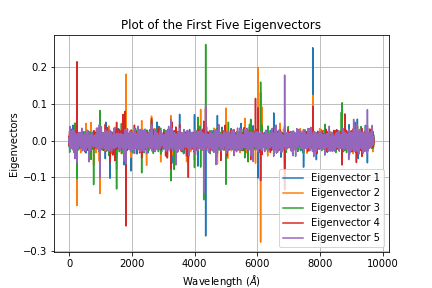
\includegraphics[width=0.7\textwidth]{eigenvector_plots.png}
			\caption{A plot of first 5 eigenvectors of the data }
			\label{fig:eigenvector_plots} 
		\end{center}
	\end{figure}

We can see that the original flux can be written as the mean spectrum + $c_{i}$ * eigenspectra * original normalization. Hence, $flux\_res$ equals $c_{i}$ * eigenvalues calculated. To get the coefficient values, they were projected on the eigenvalue basis. A plot of $c_{0}$ against $c_{1}$ and $c_{2}$ is as shown in Figure \ref{fig:c0_vs_c1_and_c2}.

	\begin{figure}[!htb]\begin{center} 
			\vspace{12pt}
			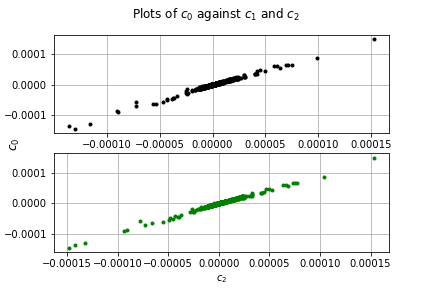
\includegraphics[width=0.8\textwidth]{c0_vs_c1_and_c2.png}
			\caption{A plot of $c_{0}$ against $c_{1}$ and $c_{2}$ }
			\label{fig:c0_vs_c1_and_c2} 
		\end{center}
	\end{figure}

For the squared residual errors, $N_{c}$ was varied from 1 to 20 in steps of 1 and plotted. The result is as shown in Figure \ref{fig:rms_vs_nc}. For $N_{c}$ = 20, we see that the rms residual error is about 1.5.

	\begin{figure}[!htb]\begin{center} 
		\vspace{12pt}
		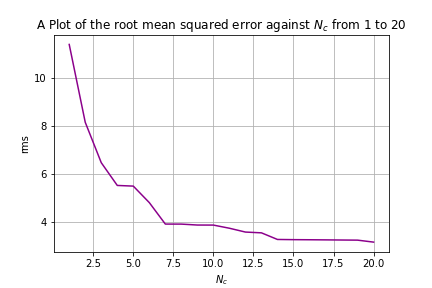
\includegraphics[width=0.8\textwidth]{rms_vs_nc.png}
		\caption{A plot of rms error against nc = 1 to 20}
		\label{fig:rms_vs_nc} 
	\end{center}
\end{figure}
	
\end{document}